\section{Particle physics instrumentation}

The use of a new detector technology in an experiment is the result of a development cycle that includes different types of activities, from generic R\&D activities, R\&D activities guided by the needs of future projects, 
focused R\&D activities for an approved experiment, production/industrialization and installation/commissioning of the technology.  As illustrated in Fig.~\ref{fig:RandD}, the work leading up to the HL-LHC detector upgrades indicates that the development cycle of a new technology is typically a decade or more.  It is therefore important for the community to plan ahead and ensure that appropriate support exists for all stages of a technology development cycle.  In 2018, an ECFA survey~[ID68] of the particle physics community found that 87\% of respondents reported engagement in R\&D activities, and that 75\% of these activities were carried out within the context of  present/future experiments (e.g. ATLAS, CMS, FAIR, etc.), 18\% within a consortium (e.g. AIDA, RDx, etc.), and 7\% of the activities were identified as generic R\&D. Looking ahead, the key to enabling new discoveries will be the community's ability to maintain an appropriately diversified portfolio of different types of R\&D activities that can evolve over time to adapt to the needs of the community.  For example, as HL-LHC upgrade activities move into construction and commissioning, it is imperative that the community maintains momentum in R\&D activities with a focus on solving the known technological challenges of the next generation of experiments. 




\begin{figure}
\begin{center}
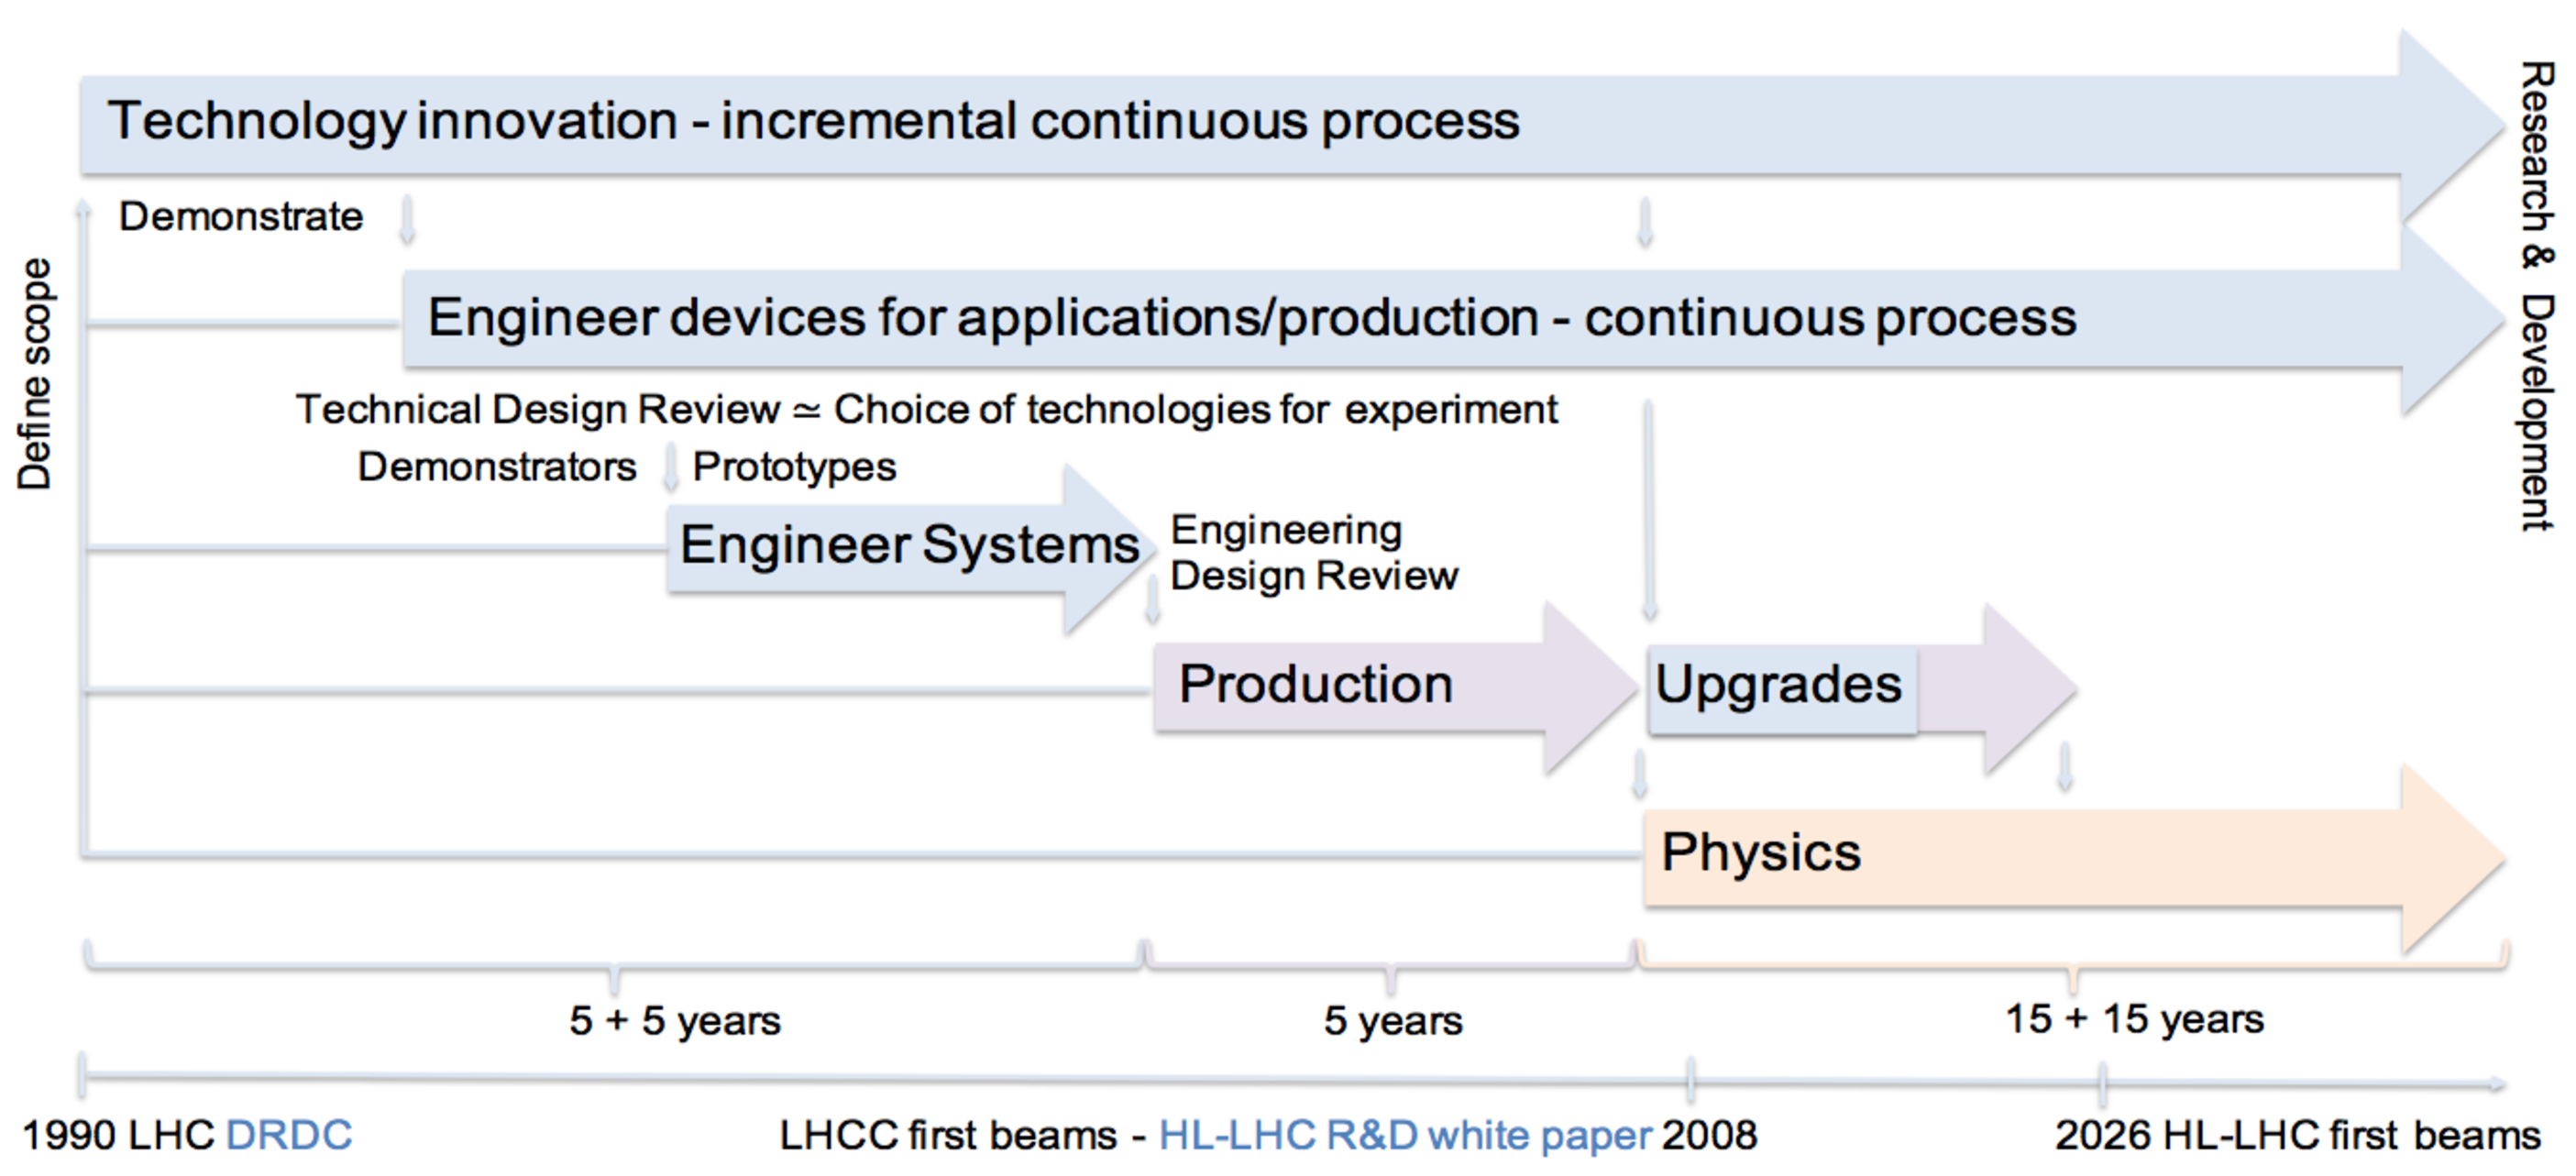
\includegraphics[width=0.99\textwidth]{Instrum/img/RandD-timeline.pdf}
\caption{\label{fig:RandD} Illustration of the typical timescale involved in the technology development cycle of particle physics experiments leading up to HL-LHC~\cite{bib:DC-talk}.}
\end{center}
\end{figure}



%-------------------------------------------
\subsection{Challenges and technologies for next generation experiments}
\label{sec:detector:challenges_technologies}
Next generation experiments include colliders as well as fixed target and beam dump facilities, together with dedicated projects for elusive particle searches. Some of the proposed programs exploit synergies between particle physics and other fields, in particular astro-particle physics and cosmology.  While the landscape of these proposed next generation experiments is broad in terms of both physics goals and detector technologies, the technological challenges are well-defined~\cite{bib:LS-talk}. These include, depending on the physics goals and experimental conditions, micron scale spatial resolution and low mass, pico-second hit time resolution, high-performance photodetectors (also operating at cryogenic temperature and low dark current), radiation tolerance, large number of channels, high readout speed, and large sensitive area at low cost. 
Moreover, the need for combined features (4D tracking, 5D imaging) becomes more and more urgent.  The time scales spanned by these future programs, ranging from few years to decades, constitutes a challenge in itself, in addition to the complexity and diversity of the required technologies.

Recent R\&D efforts have already highlighted promising technologies, some of which can apply to different detectors through specific engineering developments~\cite{bib:FS-talk}. Table~\ref{tab:tech} provides a summary of some of these promising technologies and their possible specific applications to address future experimental challenges.

%\BV{need to add a line about system integration, cooling mechanics readout electronics, software, common ancillary components, etc.}


\begin{table}
   \caption{Summary of promising technologies and their possible specific detector applications to address experimental challenges of approved and future projects.}
    \centering
%   \noindent\begin{minipage}{\textwidth}
    \begin{tabularx}{\textwidth}{>{\raggedright}XY|Y|Y|Y|Y|} 
     \multicolumn{1}{c}{} & \multicolumn{5}{c}{Technologies} \\ \hhline{~=====}
     \multicolumn{1}{c|}{} & Solid state & Gas & Scint. & \makecell{Noble liquid } & Cerenkov  \\ \hhline{~=====}
     \noalign{\medskip}\noalign{\smallskip}
%\multicolumn{6}{c}{}\\ %\hline
     %-----------------------------
     Vertex /\newline Tracker & 
     \multicolumn{5}{l}{\makecell[l]{{\bf Challenges}: high spatial resolution, fast/precise timing, rad. hardness, low\\mass, 4D tracking, high rate/occupancy.}} \\ \cline{2-6}
     \multicolumn{1}{c|}{} & \makecell{3D sensors,\\ (D)MAPS~\ref{f1}, \\LGAD~\ref{f2},\\ (HV-)CMOS~\ref{f3}}  & 
     \makecell{TPC~\ref{f4}} & \makecell{SciFi~\ref{f5} +\\ SiPM~\ref{f6}} & &  \\ \cline{2-6}
    \noalign{\medskip}\noalign{\smallskip}
     %
%     \multicolumn{6}{c}{}\\ 
    %-----------------------------
     Calorimeter &      \multicolumn{5}{l}{\makecell[l]{{\bf Challenges}: high granularity, radiation hardness, large volume, excellent\\hit timing, PFA/dual-read. capability, 5D imaging.}}\\ \cline{2-6}
     \multicolumn{1}{c|}{} &
    \makecell{Si-pad \\ sampling} & \makecell{RPC~\ref{f7} or\\ MM~\ref{f8} \\ sampling} & \makecell{Tile/fibers +\\ SiPM sampl., \\ homogeneous \\ crystals\\ (e.g. LYSO)} & \makecell{LAr\\ sampling} & \makecell{quartz fibers\\ sampling in \\ dual-readout} \\  \cline{2-6}
    \noalign{\medskip}\noalign{\smallskip}
%    \multicolumn{6}{c}{}\\ 
    %-----------------------------
     Muon det. & \multicolumn{5}{l}{\makecell[l]{{\bf Challenges}: large area, low cost, spatial resolution, high rate.}}\\ \cline{2-6}
    \multicolumn{1}{c|}{}  & &
    \makecell{MPGD~\ref{f9}, \\RPC, \\ sTGC~\ref{f10}} & & &  \\  \cline{2-6}
    \noalign{\medskip}\noalign{\smallskip}
%    \multicolumn{6}{c}{}\\ 
     %-----------------------------      
     PID &  \multicolumn{5}{l}{\makecell[l]{{\bf Challenges}: high photon detection efficiency, ultra-fast photodetectors,\\ large area photodetectors, thinner radiator.}}\\ \cline{2-6}
    \multicolumn{1}{c|}{}  & 
    \makecell{LGAD} & \makecell{TPC, RPC} & \makecell{MRPC~\ref{f11} } & & \makecell{RICH~\ref{f12},\\ TOF~\ref{f13},\\ TOP~\ref{f14},\\ TORCH~\ref{f15}}  \\  \cline{2-6}
    \noalign{\medskip}\noalign{\smallskip}
%          \multicolumn{6}{c}{}\\ 
     %-----------------------------
     Neutrino /\newline Dark Matter & \multicolumn{5}{l}{\makecell[l]{{\bf Challenges}: high photon detection efficiency, very large volume,radio \\ purity, cryogenic temperature, large area photodetectors.}} \\ \cline{2-6}
    \multicolumn{1}{c|}{}  & 
     \makecell{Si, Ge} & \makecell{TPC} & \makecell{liquid scint., \\ scint. tiles /\\ bars} & \makecell{single/dual-\\phase LAr, \\ LXe} & \makecell{water/ice + \\ mPMT~\footnote{multi-anode Photo-Multiplier Tube} }\\  \cline{2-6}\noalign{\bigskip}\cline{1-2}
%
     \multicolumn{3}{@{}p{0.49\textwidth}@{}}{%
       \raggedright\footnotesize\vspace{-0.3cm}
        \begin{enumerate}[ref=\textsuperscript{\arabic*},parsep=-3pt]
        \item (Depleted) Monolithic Active Pixel Sensor\label{f1}
        \item Low Gain Avalanche Detector\label{f2}
        \item (High Voltage CMOS)\label{f3}
        \item Time Projection Chamber\label{f4}
        \item Scintillating Fiber tracker\label{f5}
        \item Silicon Photomutiplier\label{f6}
        \item Resistive Plate Chamber\label{f7}
        \item MicroMegas detector\label{f8}
        \end{enumerate}} &
        \multicolumn{3}{@{}p{0.49\textwidth}@{}}{%
        \raggedright\footnotesize\vspace{-0.3cm}
        \begin{enumerate}[ref=\textsuperscript{\arabic*},parsep=-3pt]
        \setcounter{enumi}{8}
        \item MicroPattern Gaseous Detectors\label{f9}
        \item small-strip Thin Gap Chambers\label{f10}
        \item Multi-gap Resistive Plate Chamber\label{f11}
        \item Ring-imaging Cherenkov detector\label{f12}
        \item Time-Of-Flight detector\label{f13}
        \item Time-Of-Propagation counter\label{f14}
        \item Timing Of internally Reflected CHerenkov photons\label{f15}
        \end{enumerate}}
    \end{tabularx}
%   \end{minipage}
    \label{tab:tech}
\end{table}


Hybrid and monolithic pixel sensors for vertex and tracking detectors achieve high resolution through high granularity, low material, radiation resistance and high data rate~\cite{Garcia-Sciveres:2017ymt}. 
Monolithic Active Pixel Sensors (MAPS), in particular, initially developed for test-beam infrastructures and then adapted to the needs of high-energy physics experiments, 
have found applications in HL-LHC detector upgrades (ALICE [ID110, ID46], ATLAS~\cite{MOUSTAKAS2019604}) and are subject to process optimization for next generation experiments (CLIC~\cite{Dannheim:2673779}).
This technology is promising for its intrinsic possibility of reducing the thickness of sensors while maintaining high performance and is suited for large area assembly at low production cost.
A new avalanche silicon detector concept with a low gain, known as a Low Gain Avalanche Detector (LGAD), seems to be a favourable option to achieve, with a given pitch, the time resolution of 30~ps~\cite{Currás:2673324}. 
However, further effort is necessary to be able to achieve the combination of required performance. 
The trend towards monolithic technologies also tends to blur the boundaries with ancillary components, such as read-out circuitry, and special care must be taken in optimizing them in combination with the sensitive components.

Present and future challenges in calorimetry include excellent photon detection, high granularity, radiation hardness, large volume, and ultimately the possibility of exploiting either the particle flow~\cite{Sefkow:2015hna, THOMSON200925} or the dual read out approach~\cite{RevModPhys.90.025002}.
Research and development in the field has resulted in the use of many different technologies, depending on the application~\cite{Sefkow:2015hna}: crystals, scintillator-based sampling, silicon-based sampling, and liquid noble gas calorimeters [ID16].
Homogeneous, shashlik-type~\cite{shashlik} and spaghetti-type~\cite{Acosta:1991ap} calorimeters are considered for the LHCb electromagnetic calorimeter upgrade, while a technology similar to the ATLAS tile calorimeter is under investigation for the hadronic barrel calorimeter of an \FCChh detector. The baseline choice for an electromagnetic calorimeter for a \FCChh detector is instead based on liquid-argon technology, which was also recently considered for a detector for \FCCee.
Another option being investigated for \FCCee is the dual readout fiber calorimeter.
A silicon-tungsten calorimeter is proposed for \CLIC, the CLD~\cite{CLD} detector for \FCCee and is a promising option for \FCChh. Research and development for this technology will profit from the experience of the CMS High Granular Calorimeter (HGCal) for HL-LHC.

Particle identification is crucial for flavour physics, with the biggest challenge for the proposed future detectors being an extreme timing resolution.
The BelleII experiment at SuperKEKB [ID11] features a RICH with quartz radiator (Time-Of-Propagation or TOP) in the barrel region, which reaches a precision in the time of propagation of the order of 40~ps~\cite{Abe:2010gxa}. 
The Cherenkov technology is considered also for the LHCb detector upgrade, which features a RICH detector with a time resolution down to 10~ps and a TORCH (Time Of interally Reflected
CHerenkov light) detector with a time resolution close to 70~ps per photon resulting in an effective time resolution of 15~ps per track~\cite{Aaij:2244311}.

In the realm of gaseous detectors, Micro Pattern Gas Detectors (MPGDs [ID87]) have proven successful in many LHC experiments (e.g. GEMs, Micromegas) and are foreseen for HL-LHC detector upgrades. They remain a valid asset for addressing future experimental challenges such as high granularity and precise timing.
Glass RPC with semi-digital readout have been designed to be used as part of a hadronic calorimeter for ILD~\cite{Grenier_2014}.

For all types of particle detectors, the integration of advanced electronics and data transmission functionalities plays an increasingly important role and is a significant challenge in itself. Advances in enabling microelectronics and optoelectronics technologies are driven by industry.  Technologies used in particle physics often lag behind industry by many years, at the risk of becoming obsolete.  
The use of new microelectronic technologies for particle physics applications has a high development cost and long learning and qualification time. In this context it is important to focus on a few technology nodes (e.g. 65 nm, 28 nm) and ensure community support for design tools and foundry submissions through international coordination programs. 
%For the development of particle physics applications expensive design tools and in-depth expert knowledge are needed. In this context it is important to focus on a few technology nodes (e.g. 65 nm, 28 nm) and maintain the support for design tools and foundry submissions through large high-energy physics institutes or consortia.
Rapid development in FPGA processor power and I/O bandwidths are also enabling complex online feature extraction and increased readout flexibility; however, this comes at a cost of increased firmware development complexity which requires high level expertise.

Future experimental projects also face a large number of diverse engineering challenges, for example, in the areas of system integration, power distribution, cooling, mechanical support structures and production techniques.  Concerning mechanics and cooling infrastructures, depending on hadronic or leptonic colliders, the general requirements span from high radiation hardness to low mass and large dimension. Gas and micro-channel cooling is considered, when possible, for tracking systems.  Carbon fibre cryostats and ultrathin superconducting magnets are also being investigated.

With such plethora of options for technological development, it is mandatory to keep in mind some of the lessons learned from past R\&D~\cite{bib:DC-talk}. First, it must be recognized that efforts in R\&D activities are never loss, i.e.\ even if a technological innovation is not retained for a specific experimental program, it is nevertheless available for other projects.   Furthermore, in the context of R\&D activities guided by the needs of future projects, technological specifications must be well-defined and documented, and need to consider all aspects of the final applications: compatibility with other systems and their global performance, operating conditions including their uncertainties and required margins, production capabilities and costs. For common components developed to address the needs of several detectors and experiments, anticipating the implementation of different configurations is particularly important. 
Thorough definition and documentation of test protocols, including test conditions as close as possible to final operation, and earliest possible start of radiation tolerance tests are fundamental to minimize risks.
Finally, given that components may be discontinued by vendors or become prohibited due to new legislation, the market behaviour must be constantly monitored and some degree of diversity of solutions must be maintained.

%-------------------------------------------
\subsection{Generic detector R\&D}

Generic detector R\&D refers to research activities that seek to push back the limits of technology, and is not uniquely driven by the needs to fulfill specific experimental requirements.  Since generic detector R\&D has the potential to bring about tool-driven revolutions, it is essential that the community maintains the ability to carry out these types of research activities, even through the design, planning and execution of large experimental projects.  An example of this is the outcome of continued improvements made in solid state sensors which has led to the possibility to add timing detectors to LHC experiments upgrades; an improvement that was not originally foreseen and that is now opening up the ability to achieve better pile-up rejection.  

Generic technology innovation often emerges from synergies within the field of particle physics, with other fields of science, or with industry, and in most cases, is an incremental, continuous and long term process.  Furthermore, generic R\&D, by itself, can typically be costly and often requires access to various specialized infrastructures (c.f.\ Sect.~\ref{sec:detector:infrastructure}).  As a result, programs such as AIDA2020 and ATTRACT, play an important role in enabling and supporting generic R\&D activities. %(c.f. Sections~\ref{sec:detector-synergies} and \label{sec:detector:infrastructure}).  
It is therefore important to ensure that these types of program be appropriately supported and have also the ability to expand, as needed, in order to preserve and stimulate the community's potential for innovation. 



%--------------------------------------------------------
\subsection{Test facilities, infrastructures and tools}
\label{sec:detector:infrastructure}


The development of novel particle physics
instruments requires specialized infrastructures, tools and access to test
facilities that all come at a substantial
costs.  National labs and large institutions play a central and 
important role in support for the community
by providing access to, and user support for, these facilities, infrastructures and tools.  

\paragraph*{Test beam and irradiation facilities}
Test beam facilities are vital for the characterization, calibration and commissioning of new instruments.  A list of test beam facilities in the world currently available to the particle physics community is presented in Table~\ref{tab:testbeam}.  These facilities offer different particle species, energies and beam structures that are complementary to each other.   In the past few years, the demand for access to the largest test beam facilities such as those at CERN, DESY, Fermilab and SLAC has remained high.  The CERN test beam facilities, for example, are at present used at full capacity.  It is expected that the development of instrumentation for approved and future projects will maintain, even possibly increase, the need of the community to have access to these types of facilities.  Yet, the future medium to long term availability of some of the test beam facilities currently used by the community is at present uncertain.  Furthermore, parts of these facilities, for example at CERN, are also aging and will require adequate maintenance and/or upgrade in the coming years to continue to support the community.  


\begin{table}
    \caption{List of test beam facilities in the world, as of May 2019. Only beam lines with beams of energies higher than 100~MeV are included [Courtesy of C. Rembser and H. Wilkens].}
    \centering
    \footnotesize
    \begin{tabularx}{\textwidth}{XYYYY} \hline\hline
    Laboratory & Number of beam lines & Particles & Energy  & Availability \\ \hline\hline
    %-------------------------------
    CERN/PS\newline (CH) & 
    2 & 
    $\rm e, h, \mu (sec.)$ & 
    0.5 - 10~GeV &
    \multirow{2}{2.5cm}{9 months per year continuous except winter shutdown, typical duty cycle \\ PS$\sim$ 1-3\% \\ SPS 20-40\%}
    \\  \cline{1-4}
    %---------------------------------
    CERN/SPS\newline (CH) & 
    4 & 
    p(prim.) \newline e,h,$\mu$(sec.)\newline e,h(tert.) \newline Pb ions (prim.) \newline other ion species \newline (out of fragmented primary Pb ions)  &
    400~GeV\newline 10-400~GeV \newline 10-200~GeV \newline \newline 20-400~GeV\newline proton equiv.\newline (z=1) & 
    \\ \hline
    %---------------------------------
    Frascati\newline DAFNE BTF\newline (IT) &
    2 &
    $\rm e^+/e^-$ both prim. and sec. &
    25-750~MeV\newline Rep. rate 50~Hz\newline 1-40~ns\newline $\rm 1-10^{10}$~part./pulse &
    Typically 25-35 weeks/year \\ \hline
    %---------------------------------
    DESY\newline (D) & 
    3 &
    $\rm e^+,e^-$(sec.) &
    1-6~GeV\newline 6.3~GeV\newline max 100~kHz &
    11 months per year,\newline duty cycle ~ 50\% \\ \hline
    %---------------------------------
    ELPH (Sendai)\newline (JP) &
    2 &
    photons (tagged)\newline $\rm e^+,e^-$(conv.) &
    0.7-1.2~GeV \newline0.1-1.0~GeV\newline beam rate < 500~kHz\newline (typ. rate: 2~kHz) &
    2 months/year \\ \hline
    %---------------------------------
    FERMILAB FTBF \newline (US) &
    2 &
    p(prim.) \newline e,h,$\mu$(sec.)\newline h(tert.) &
    120~GeV\newline 1-66~GeV \newline 200-500~MeV &
    24~hrs/day, duty cycle 6\% \\ \hline
    %---------------------------------
    IHEP (Beijing)\newline (CH) &
    2 & 
    e(prim.)\newline e(sec.) \newline p,$\pi$(sec.) &
    1.1-2.5~GeV\newline 100-300~MeV \newline 0.4-1.2~GeV &
    3 months/yr, duty cycle depends on BEPCII operation mode \\ \hline
    %---------------------------------   
    IHEP (Protvino) \newline (RU) & 
    5 & 
    p(prim.)\newline p,K,$\pi,\mu$e(sec.)\newline C-12(prim) &
    70~GeV\newline1-45~GeV\newline 6-300~GeV &
    2 months/yrs\newline duty cycle(U-70 machine) 15-30\% \\ \hline
    %---------------------------------
    PSI piE1, piM1, etc. \newline (CH) &
    2-4 &
    $\rm \pi^{\pm},\mu^\pm,e^\pm$,p &
    50-450~MeV\newline rate < $10^9$~Hz\newline 20~ns structure, continuous beam at very high rate &
    6-8 months/yr \\ \hline
    %---------------------------------
    SLAC\newline (US) &
    0 & 
    e(prim.)\newline e(sec.) & 
    2.5-15~GeV\newline 1-14~GeV &
    9 months/yr \newline duty cycle 50\% \newline [No beam in 2019] \\ \hline
    %---------------------------------
    SPRING-8\newline Compton Facility\newline (JP) &
    1 & 
    photons(tagged)\newline $\rm e^\pm$(conv.) &
    1.5-3.0~GeV\newline 0.4-3.0~GeV &
    $>$60 days/yr \\ \hline
    %---------------------------------
    University of Bonn\newline ELSA \newline (D) &
    1 &
    $\rm e^-$ &
    1.2-3.2~Gev\newline rate ~ 500~Hz-1~GHz &
    Upon request, \newline typ. $\sim$ 30 days/yr \\ \hline
    %---------------------------------
    University of Mainz \newline MAMI \newline (D) &
    3 &
    $\rm e^-$ \newline photons &
    $\rm E_{e^-,\gamma}$ < 1.6~GeV \newline $\rm e^-$ intensity < 100~$\mu$A &
    Upon request, \newline typ. $\sim$ 30 days/yr \\ \hline
    \end{tabularx}
    \label{tab:testbeam}
\end{table}



Irradiation facilities are used to characterize the radiation hardness, aging effects and performance of detectors, electronics components, systems and materials, under high particle flux and fluence such as those expected at accelerators and in accelerator-based experiments.  Table~\ref{tab:irradiation} summarizes information about a representative sample of irradiation facilities in the world used by the particle physics community for the testing and qualification of detector and accelerator components.  In addition, many other facilities are available to the community and information about these facilities can be found in the AIDA2020-supported world-wide database of irradiation facilities~\cite{bib:db}.  Current irradiation facilities fulfill, and have been optimized in some cases for, the HL-LHC radiation environment.  The particle fluence expected at some of the future accelerator projects will however be more than a factor of 10 larger (e.g. fluence of $10^{17}$ particles/$\rm cm^2$ at \FCChh for 30~ab$^{-1}$).  In the future, the testing of materials, devices, systems and electronics under this type of extreme radiation environment will be critical and require access to irradiation facilities with increased particle fluxes, larger radiation areas for simultaneous tests of many components, and longer testing campaigns.  


\begin{table}
    \caption{Representative list of some of the different types of irradiation facilities in the world commonly used by the particle physics community for the testing and qualification of detector and accelerator components~\cite{bib:cern-radiation,bib:irradiation-talk}. This list is not an exhaustive list since irradiation services can be sometimes supplied by some member institutions of an R\&D project, the community makes use of industrial services or of medial accelerators for reasons of convenience, availability, etc., and in other cases, irradiation must be performed with specific particles/energies.
    Several other facilities are available to the community and can be found in the AIDA2020-supported world-wide database of irradiation facilities~\cite{bib:db}.}
    \centering
    \footnotesize
%    \begin{tabularx}{\textwidth}{p{2.5cm}p{1.8cm}YY} \hline\hline
%\begin{tabularx}{\textwidth}{p{2.5cm}SYY}
\begin{tabularx}{\textwidth}{SSYM}\hline\hline
    Access provider\newline and infrastructure  & Particles & Energy, flux, etc.  & Availability \\ \hline\hline
    %-------------------------------
%    CERN/VESPER\newline (CH) &
%    $\rm e^-$ &
%    50-250~MeV\newline average flux $\rm \sim 1\times 10^8 e/cm^2/s$ &
%    8-9 months/yr \\ \hline
    %-------------------------------
    CERN/IRRAD \newline (CH) &
    p &
    24~GeV\newline flux: $\rm 1-3\times 10^{10}~p/cm^2/s$ &
    May-November \newline [Closed during LS2] \\ \hline
    %-------------------------------    
%    PSI/PIF \newline (CH) &
%    p &
%    5-230~MeV \newline max current 2-4~nA\newline rate < $10^9$~Hz\newline typ. flux $\rm 10^8 p/cm^2/s$ for wide beam\newline energy,beam spot, flux selectable by user &
%    11 months/yr\newline mostly during weekends \\ \hline
    %-------------------------------  
    KIT/KAZ\newline (D) &
    \makecell{p\\ \\ \\ x-ray}&
    25.3~MeV \newline current 2~$\mu$A\newline flux$\rm\sim 2.5\times 10^{13}~p/cm^2/s$ \newline dose rate up to 18~kGy/h&
     \\ \hline
    %-------------------------------  
    UoB/MC40\newline cyclotron\newline (UK) &
    p &
    up to 40~MeV, typ. 27~MeV \newline current < 2~$\mu$A, typ. 0.1-0.5~$\mu$A \newline flux $\rm\sim 10^{13} p/cm^2/s$ &
     \\ \hline
    %------------------------------- 
    CERN/CC60 \newline (CH)&
    $\gamma$ &
    1.17~MeV, 1.33~MeV\newline (10~TBq $\rm {}^{60}Co$ source)\newline $\rm\sim~3~Gy/h$ at 1~m & 
    All year
     \\ \hline
    %------------------------------- 
    CERN/GIF++ \newline (CH) &
    \makecell{$\gamma$\\ \\ \\ \\ (+$\mu$)} &
    0.662~MeV\newline (14~TBq $\rm {}^{137}Cs$ source)\newline dose-rate $\sim$0.5~Gy/h at 1~m\newline selectable flux\newline typ. 100~GeV, $\rm \sim 10^4$ part./spill & All year \newline (+ 6-8 weeks/yr \newline of SPS operation)
    \\ \hline
     %------------------------------- 
     CERN/CHARM \newline (CH) &
     \makecell{mixed-field \\ (24~GeV p \\ on Cu/Al \\ target)} & n: thermal - HE\newline HEH: > 100~MeV\newline Lateral: $\rm 10^7-10^{10}~HEH/cm^2/h$\newline Long.:$\rm 10^8 - 10^{12}~HEH/cm^2/h$\newline  homogeneous field over $\rm \sim 1~m^2$ &
     May-November \newline [Closed during LS2]
     \\ \hline
     %------------------------------- 
     UCL/CRC \newline (BE) &
     \makecell{heavy \\ ions} &
     high LET or high penetration cocktail\newline flux $\rm\sim$ few - $\rm 10^4~part/cm^2/s$ & 
     \\ \hline
     %------------------------------- 
     JSI/TRIGA\newline reactor \newline (SI) &
     n &
     fast \& thermal,\newline flux $\rm 1-4\times 10^{12}~n/cm^2/s$\newline thermal, regenerated fast,\newline flux $\rm < 5\times 10^8~n/cm^2/s$ &
     \\ \hline
     %------------------------------- 
     Los Alamos/\newline Sandia\newline (US) &
     \makecell{p \\ \\ n\\ \\ $\gamma$} &
     800~MeV, \newline $\rm 5\times 10^11$~part./pulse at 1~Hz \newline 0.1~MeV to > 600~MeV, \newline $\rm 10^6~n/cm^2/s$ above 1~MeV per pulse \newline dose rate $10^{-8}$ - 10~Gy/s &
     \\ \hline
    \end{tabularx}
    \label{tab:irradiation}
\end{table}




The recent and ongoing testing campaign of novel instruments in preparation for HL-LHC has shown that the time availability to testbeam and irradiation facilities can in some cases be a limiting factor.  While access to many facilities are available to the community through transnational access programs such as that provided by AIDA2020, others are user-paying facilities.  The ability to make extensive use of these facilities also importantly depends on the quality of user and technical support, as well as the availability of high-quality beam instrumentation and test set-ups.  An ECFA survey~[ID68] of the particle physics community in 2018 found that the ability to access testbeam/irradiation facilities and the quality of their infrastructures were generally very good.  Continued and coordinated support of a European network of test beam and specialized irradiation facilities, including user support, is of the utmost importance for the community.

Established in 2014, the CERN neutrino platform provides the neutrino community with support for detector R\&D, tests, construction, as well as access to a charged particle test beam infrastructure.  This initiative is an important complementary contribution to the US and Japanese neutrino programs and is providing coherence to the European neutrino community.  This type of initiative could be considered for other research topics.
\vfill

\paragraph*{Infrastructures}
Typical infrastructures required for instrumentation development
include, but are not limited to, clean rooms, probe stations,
bonding/packaging tools, radioactive/laser sources, 
spectro-photometer and spectro-fluorometers, specialized electronics and data acquisition equipment, equipment for impurity/dopant, content and profiles in solid 
state devices, etc. While some of this type of infrastructure can be available
at some institutions, the cost can be prohibitive to many and often can be
single-used for a particular project.  National labs and large institutions play a critical role in providing access to various specialized infrastructures required for detector R\&D.  The sharing of such infrastructures 
is important for the community.   Furthermore, efficient usage of existing
infrastructures requires the existence of platform(s) 
disseminating the information, and potentially coordinating the
infrastructures usage.  
%\vfill

\paragraph*{Specialized tools} In the development of novel technologies, the use of specialized tools is
essential to minimize, for example, the number of prototype
iterations.  These specialized tools include modelling tools, advanced
detector simulation tools, tools to estimate radiation doses, and
design and validation of electronics system and mechanical 
components.  While some of these tools are free, others have costly
licenses.  National labs and larger organizations can play an important role in
providing the community with access to, and expertise in the use of, some of these specialized tools.  
It is also important to note that the particle physics community has
also a role to play in the 
development of some of these tools (e.g.\ GEANT4~\cite{bib:geant1,bib:geant2,bib:geant3}), ensuring that the
tools meet the needs of the community.  A strong synergy exists between access to test beam facilities providing well-defined conditions and the ability to improve simulation models of particle interactions with materials that are important for the design of novel technologies. 


%The realization of large scale projects such as HL-LHC experimental upgrades has %shown the importance of expertise and support in areas of project management.  








%\begin{figure}
%\begin{center}
%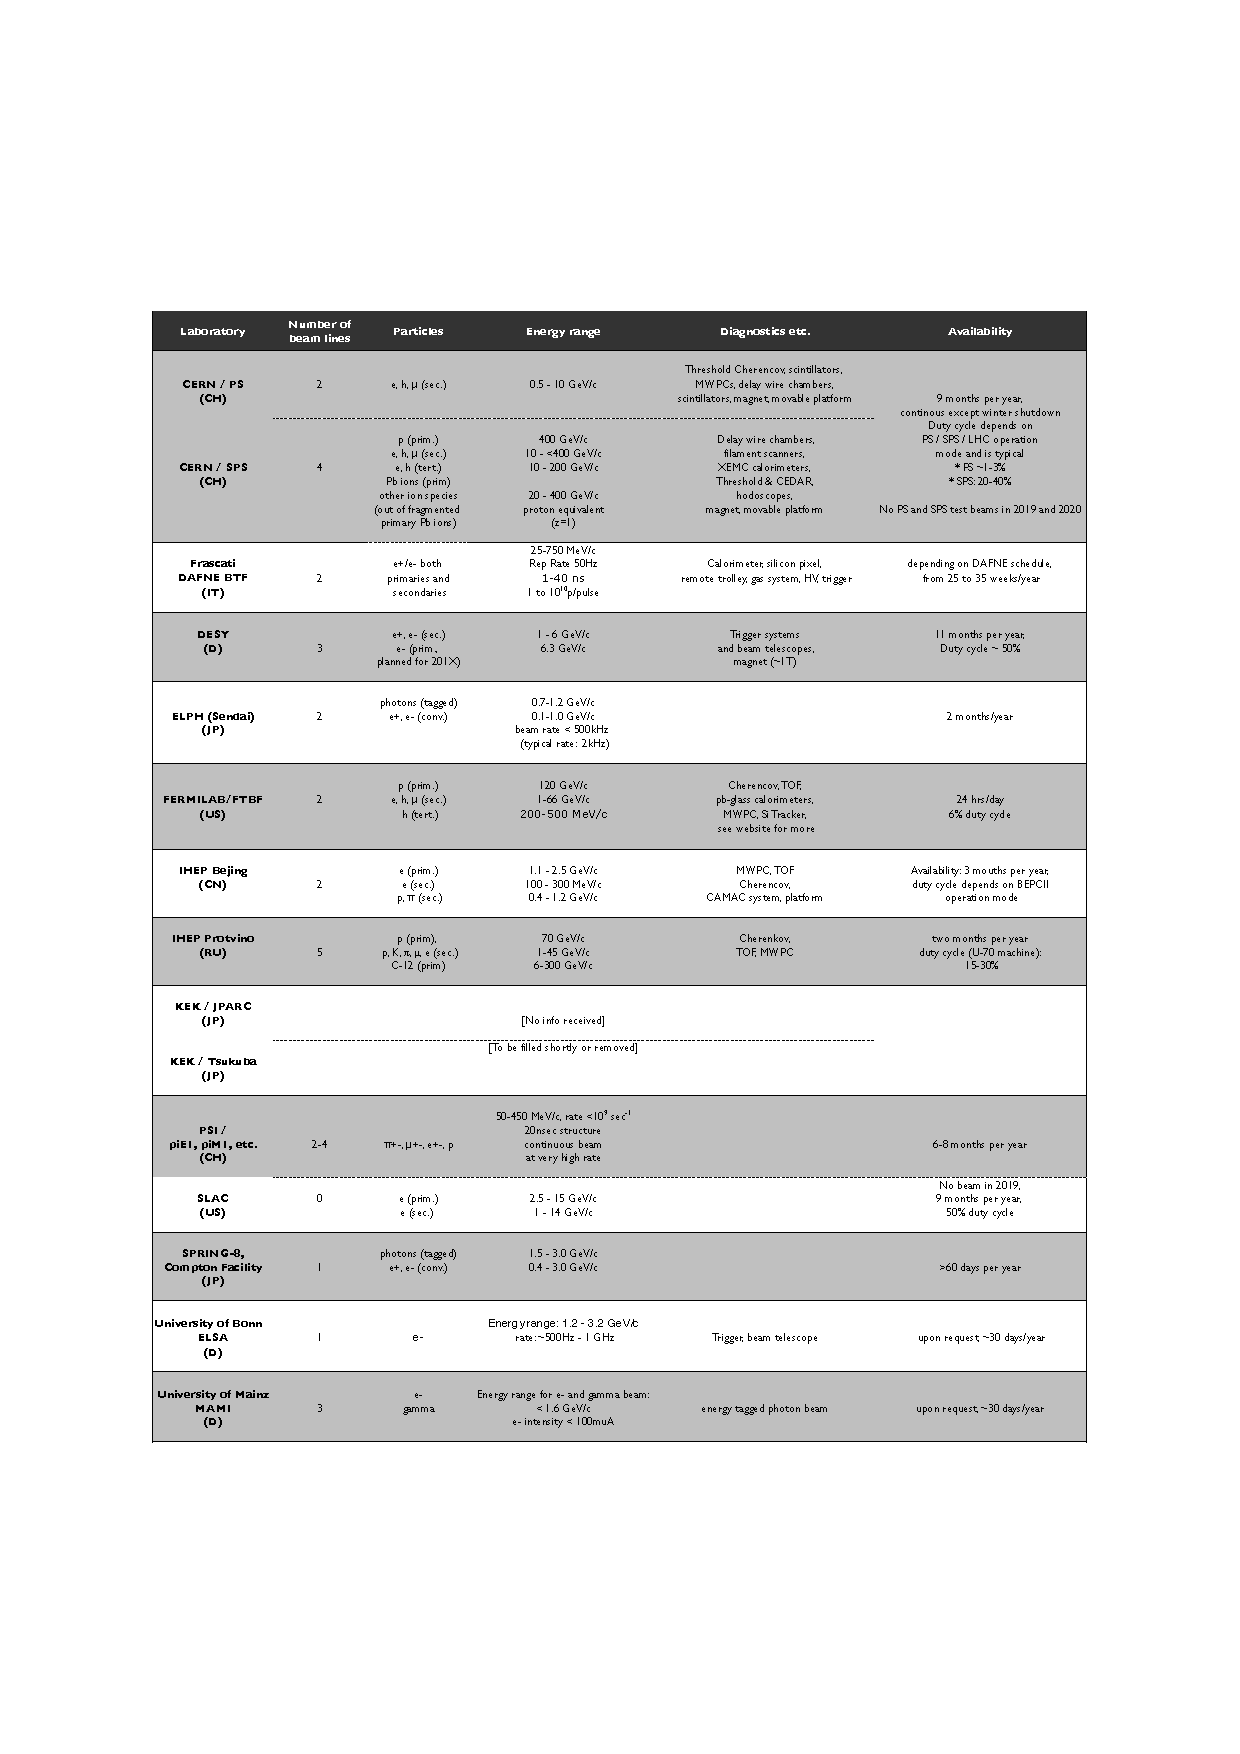
\includegraphics[width=0.95\textwidth]{section1/img/2019_testbeam.pdf}
%\caption{\label{fig:testbeam} List of test beam facilities in the world, as of May 2019. Only beam %lines with beams of energies higher than 100~MeV are included [Courtesy of C. Rembser and H. %Wilkens). \BV{Formatting of this table still under-development, suggestions welcome.}}
%\end{center}
%\end{figure}

%\begin{figure}
%\begin{center}
%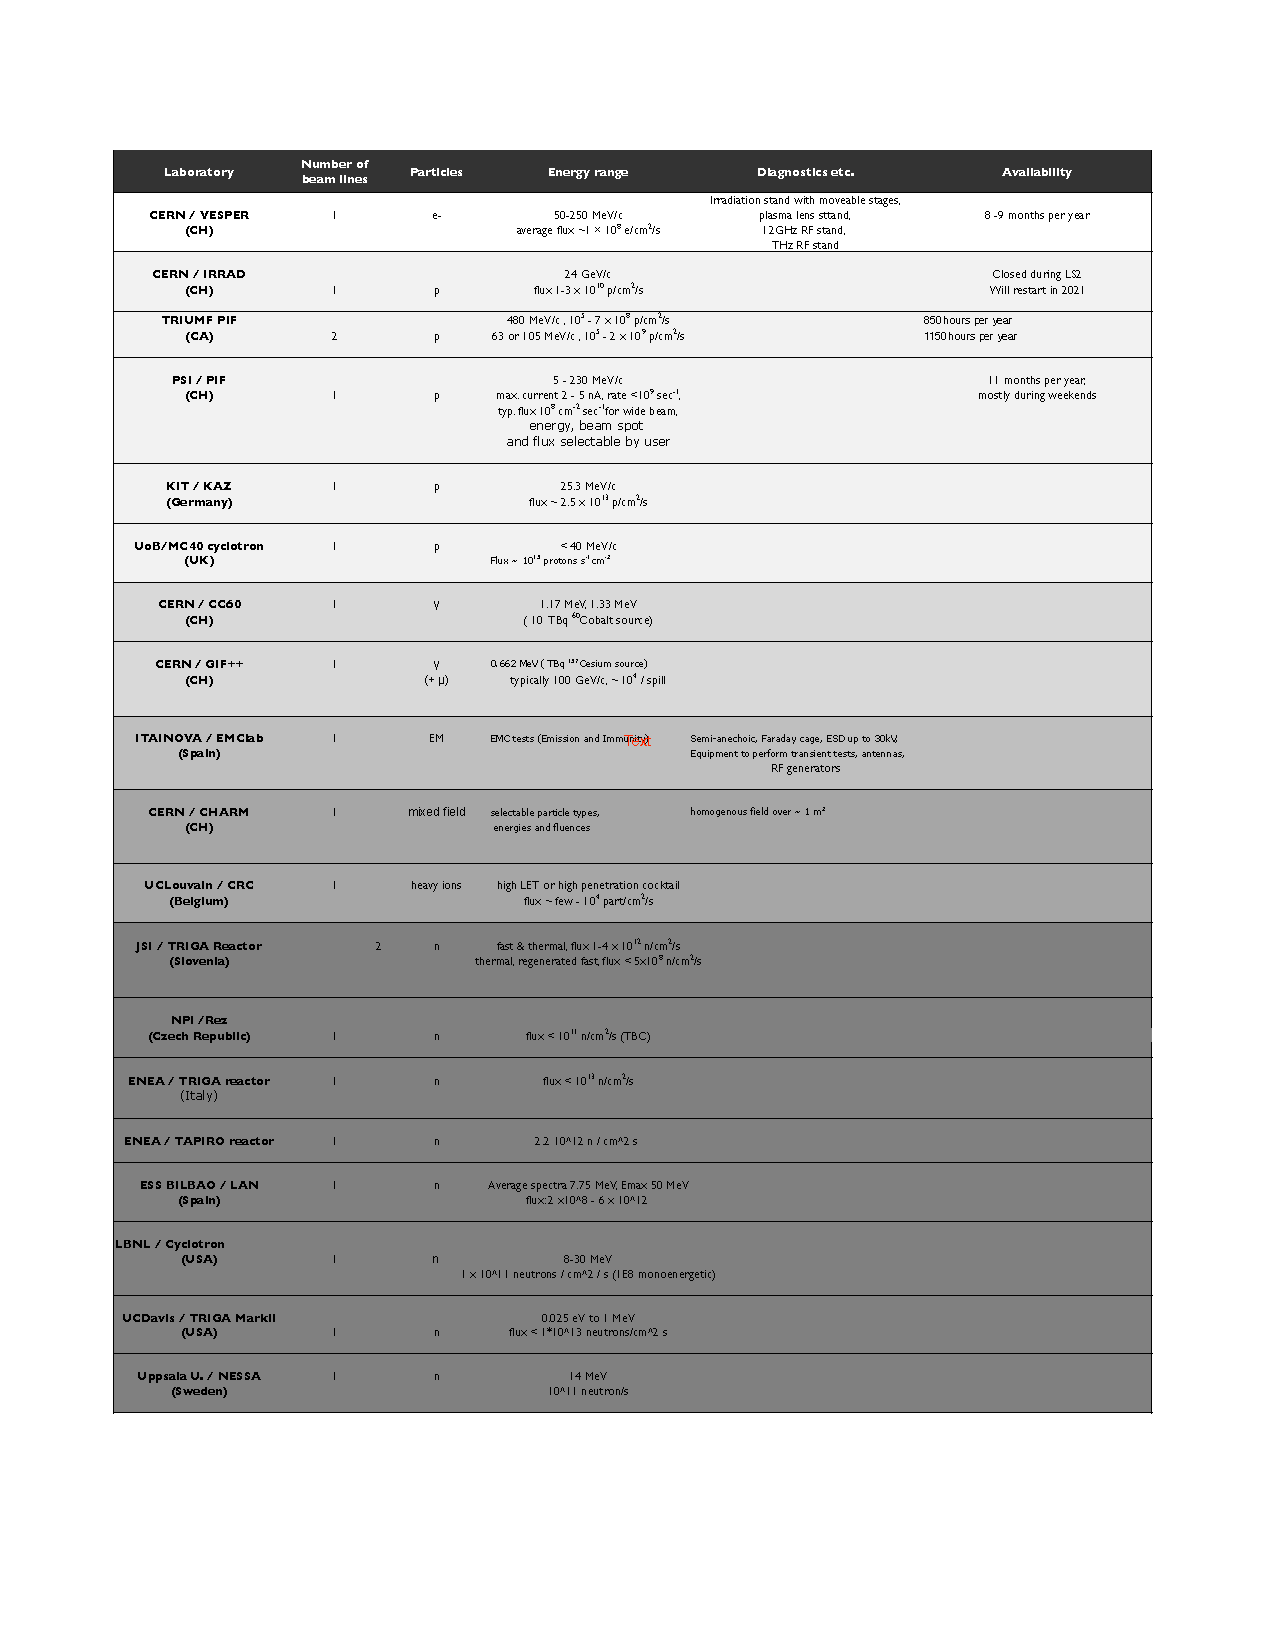
\includegraphics[width=0.95\textwidth]{section1/img/2019_irradiation.pdf}
%\caption{\label{fig:irradiation} List of some of the higher flux irradiation facilities in the %world, along with specialized facilities, commonly used by the particle physics community in recent %years. Several other facilities are available to the community and can be found in the %AIDA2020-supported world-wide database of irradiation facilities~\cite{bib:db}. \BV{Formatting of %this table still under-development, suggestions welcome.}}
%\end{center}
%\end{figure}




%\begin{table}[]
%    \centering
%    \begin{tabular}{c|c}
%         &  \\
%         & 
%    \end{tabular}
%    \caption{Give link, and summarize here only European facility,large volume capability, highest activity %}
%    \label{tab:my_label}
%\end{table}




%--Coordination - 
%-------------------------------------------------------------------------------
\subsection{R\&D coordination}
\label{sec:coordination}

Results of the 2018 ECFA survey~[ID68] of the particle physics community clearly demonstate that expertise in instrumentation R\&D is distributed over many institutions (universities, national and international laboratories).  As such, international coordination of R\&D activities is critical to maximize the scientific outcomes of these activities and make the most efficient use of resources. More specifically, the coordination of activities provides
\begin{itemize}
\item the ability to efficiently share and streamline work thereby limiting duplication of efforts,
\item opportunities for the development of, and access to, common tools, infrastructures and services,
\item access to a large network of information and worldwide expertise in different areas,
\item wide dissemination of knowledge and results,
\item unique environment for the training of the next generation of experts,
\item a visible framework for institutions.
\end{itemize}

The community has a strong track record of successful implementation of different collaborative structures used to coordinate R\&D activities.  These include, for example,
\begin{itemize}
\item CERN R\&D programs such as the DRDC and White Paper Theme 3 R\&D programs which laid the foundations for the construction and subsequent upgrades of the LHC detectors;
\item European Commission funded projects such as EUDET, AIDA, AIDA2020 and ATTRACT which provide precious support to the particle physics community to develop new devices, common ancillary electronics, beam test and irradiation facilities, and also play an important community building role in establishing coherence at the European level;
\item other R\&D collaborations (e.g.\ CALICE, ProtoDUNE) that, in some cases, have the flexibility to evolve in scope.
\end{itemize}

%Beyond the exploitation of the potential of the HL-LHC, while the experimental options at this point in time are numerous, their technological challenges are however well-defined.
Looking ahead, there is a clear need to strengthen existing R\&D collaborative structures, and create new ones, to address future experimental challenges of the field post HL-LHC. Consistent with this view, CERN has proposed a R\&D programme [ID16] that concentrates on advancing key technologies rather than on developing specialized detector applications. %This strategic R\&D program on technologies for future experiments is organized around key technologies in the areas of detectors, electronics, software, mechanics, cooling and magnets.  
Many of the developments are proposed to be be carried out jointly with external groups, also exploiting existing collaborative structures like the RD50 and RD51 collaborations, and with industrial partners.
In addition, it is generally acknowledged that the community must continue to vigorously pursue the development of future EC-funded projects, which have played a central role in enabling past R\&D activities.  
These projects all have strong leverage on matching funds. 

Some of the challenges in maintaining the community's ability to carry out detector R\&D research through collaborative structures include:
\begin{itemize}
    \item Evaluation of, and ability to secure, the appropriate level of funding.  For example, there is a feeling among some stakeholders that more funding for innovation could have enabled devices with improved performance and/or lower cost for HL-LHC (e.g.\ more radiation tolerant Crystals, SiPMs, CMOS sensors with fast readout, etc.).  In general, R\&D has high added value compared to the overall cost of the scientific programs.
    \item While collaborative structures can build on several smaller scale national and local initiatives with various funding sources, this implies that (at least some) resources are in the hand of contributing institutions.  As a result, estimating efforts needed/invested is not easy and unforeseen withdrawals of efforts can impact schedules. More formal agreements throughout different R\&D phases could help address this challenge.
    \item Maintaining effectiveness.  Experience has shown that an international independent R\&D review process of consortia and programs is important for maintaining their effectiveness and securing funding.
    \item Integration of R\&D not targeted at CERN-hosted projects.
    \item Engagement with world-wide (non-European) community.
\end{itemize}

To help address some of these challenges, it would be advantageous 
for the community to define a global R\&D roadmap that could be used to support proposals at the European and national levels.  This community roadmap could, for example, identify grand challenges to guide the R\&D process on the medium and long term timescales, as well as define technology nodes, broad enough to be used as a basis for creating R\&D platforms. 
%Furthermore, improved global coordination of efforts could be achieved by creating a central database of developments, including documentation, to be used for keeping track of ongoing activities in the community at large, to provide linkage between groups working on related topics, and to provide information on R\&D to other scientific fields and industry.



%In the 1990s, 50 CERN international R\&D programs (DRDC) were organized for the LHC preparation, mostly based on the various technical options for the detectors with a goal to select solutions for the approved experiments. 
%R\&D that did not converge to enter a detector often formed a basis for future developments. 
%In preparation of HL-LHC, CERN R\&D programs were identified with a goal of developing common technical solutions for the various experiments. CERN work packages were also created for the development of ancillary electronic components common to all detectors and experiments (ASIC technology, optical data transmission and power distribution), and for preparation of beam test and irradiation facilities. 
%(GIF++, IRRAD, CHARM \EL{need ref}). 
%This approach allowed to streamline efforts to deliver the required new techniques and common components in time for the final engineering and construction. These common programs have been very successful in the past and should be encouraged and pursued in the future. %Two fruitful examples of R\&D for ILC, CALICE for the high-granular calorimeter and the Monolithic Active pixels for tracking, were not anticipated to serve HL-LHC upgrades. However, they provided a relay to technology innovation that enabled selecting these new techniques respectively for the upgrades of CMS and ALICE. 
%Building on these successful R\&D activities, a strategic R\&D programme on technologies for future experiments has been proposed [ID16], organized around key technologies in the areas of detectors, electronics, software, mechanics, cooling and magnets. 
%Drawing a strategic R\&D road map at this point in time is challenging, since the future course of the field is just emerging. A proposed R\&D strategic plan~\cite{ID16} has identified a series of programs with appropriate balance of orientations and defined timelines, based on key technology nodes rather than specialized applications. Similarly as for HL-LHC, technological R\&D must address not only the requirement of the different sub-detectors, but also those of general services such as magnets and software. 

%In the past, European funded detector R\&D projects such as EUDET, AIDA and AIDA2020 guaranteed precious support to the high-energy physics community to develop new devices, common ancillary electronics, beam test and irradiation facilities. Moreover, they provided a unique community building role in establishing coherence at the European level.
%International R\&D programs in general offer an efficient framework to streamline work and provide common services. 
%They can build on several smaller scale national and local initiatives with various funding sources. Furthermore, experience has shown that an international independent R\&D review process of consortia and programs is important for maintaining their effectiveness and securing funding.

%Continued support is requested for detector development collaborations and consortia such as RD50, RD51, RD53, CALICE and the follow-up of AIDA, recognising enhanced productivity achieved through general networking, such as the exchange of information and methodologies, and the sharing of efforts, investments and infrastructures. Further initiatives towards similar R\&D collaborations, initiated by CERN or through new European funding programmes, are encouraged.

%Efficient R\&D coordination can be achieved by creating a central database of developments, including documentation, to be used for keeping track of ongoing activities, provide linkage between groups working on related topics, and provide information on R\&D to other scientific fields and industry.

%It should be kept in mind that R\&D has high added value compared to the overall cost of the scientific programs.
%For the successful outcome of such programs, continued funding and the efficient use of resources are critical.
%Recommendations should emerge from this European Strategy process in the shape of grand challenges for medium and longer term to address European and national funding agencies and encourage continuity in financial support.

%-----------------------------------------------------
\subsection{Synergies and opportunities}
\label{sec:detector-synergies}

Instrumentation development for particle physics is both a driver for, and a beneficiary of, progress made in other areas, within the field of particle physics, in other fields of science, and industry. 

Within the field of particle physics, technologies developed under generic R\&D programs or with the aim to address common experimental challenges often provide a boost in innovation that suits the needs of detector upgrades and/or novel designs. Examples of this include the development of liquid noble gas Time Projection Chambers (TPCs) for dark matter and neutrino experiments (DarkSide [ID62], DARWIN [ID97], DUNE [ID126, ID131]), liquid scintillator with photomultipliers (JUNO [ID19]), and pure water Cherenkov with photomultipliers (SuperKamiokande). A highly-granular electromagnetic calorimeter, addressing similar needs as the CMS electromagnetic calorimeter upgrade (HGCal), is foreseen for the Light Dark Matter eXperiment (LDMX) at eSPS [ID42, ID36]. A fast radiation-hard electromagnetic calorimeter using GAGG crystals, similar to the LHCb electromagnetic calorimeter for LHCb Upgrade II, is designed for the fixed-target experiment TauFV [ID42, ID102]. The two experiments also share the design of the TORCH particle identification detector mentioned in  Sect.~\ref{sec:detector:challenges_technologies}.

Across other fields of science, in particular with the astro-physics and cosmology communities, strong synergies for detector R\&D have been identified~\cite{bib:CDV-talk}. % in addition to synergies in "physics"
For example, the design and construction of gravitational wave interferometers (e.g.\ Einstein telescope [ID64]) will profit from developments in cryogenics and ultra-vacuum technologies driven by the needs of particle physics experiments.  Particle physics has also been the driver of important developments in the fields of medicine (e.g.\ medical imaging, radiation treatments, etc.) and biology. For example, the Medipix and Timepix chips~\cite{bib:medipix} originally developed to meet requirements of solid state tracking detectors and TPCs in particle physics have found applications in medical imaging, space dosimetry, material analysis (e.g.\ characterisation of pharmaceuticals, evaluation and synthesis of new materials, detection of counterfeit drugs). To facilitate the cross-fertilization of innovations across disciplines, the development of technology-centered R\&D programs, as well as platforms for the exchange of information and ideas, should be encouraged.
%such multidisciplinary approaches, the need for adequate platforms for the exchange of information and ideas has emerged. In this context, possible options may be the organization of joint conferences or multidisciplinary working groups.

The relationship with external partners is as bidirectional as within scientific fields. 
%\EL{The following sentence is not strictly detector only - decide what to do} Synergies can be found at different levels: particle accelerators (radiotherapy, synchrotron light sources), electrical, material and civil engineering (tunnels, power system, robotics), big data (astronomy, bioinformatics) and detector (Medipix and Timepix, MPGDs applied to radioactive waste treatment).
Products of particle physics are highly specific with relatively small and cyclic markets. Their developments and production rely on partners working in other scientific and societal fields using similar devices, particularly for imaging technologies, for electronics and mechanical systems. In some cases, collaboration and knowledge transfer with industrial partners (e.g.\ access to the bases of fabrication process, understanding the mechanisms of industrialization) are absolutely necessary for ensuring mass production and for reducing the risks of market instability.
Successful initiatives of collaboration and cooperation with industry partners (e.g.\ ATTRACT~\cite{bib:ATTRACT}, ERDIT~\cite{bib:ERDIT}) should be encouraged.
Valuable candidates for partnership range from material science laboratories, foundations or start-ups in technology innovations for relatively small productions, to medium size companies for larger productions and scientific/technical knowledge transfer (e.g.\ Hamamatsu Photonics for providing large quantities of silicon sensors for HL-LHC, TowerJazz for producing CMOS MAPs).
It is subject of debate whether involving industrial partners at an earlier stage of the scientific R\&D projects would be beneficial to particle physics. In this respect, careful thoughts must be put into regulatory matters and patent issues.

%Such an example is ATTRACT[\BV{need reference}], that brings together Europe's fundamental research and industrial communities to promote groundbreaking ideas in the field of detection and imaging technologies.
%Along the same line is the ERDIT[\BV{need reference}] platform, established to synergistically implement a common research strategy across research infrastructures involving research laboratories, academy and industry, from which evidence emerges that detector requirements and R\&D needs are converging across disciplines.